بردار گرادیان J برداری است که هر عضو آن مشتق جزئی اسکالر J نسبت به xi است.
جهت بردار گرادیان در نمودار فاز تابع به سمت بیشترین افزایش تابع است.
از این جهت استفاده از بردار گرادیان برای پیدا کردن ماکسیمم تابع عملا نسخه پیوسته الگوریتم hill-climbing است.
 در نتیجه میتوانیم الگوریتم descent gradient را مطابق زیر معرفی کنیم.

\begin{figure}[H]
    \centering
    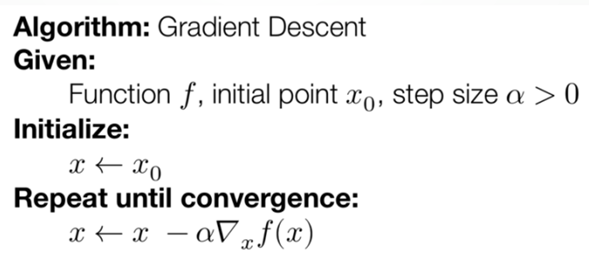
\includegraphics[width=0.5\textwidth]{source/gradient-descent.png}
    \label{fig:descent-gradient}
\end{figure}

اثبات convergence در الگوریتم descent gradient :

\begin{figure}[H]
    \centering
    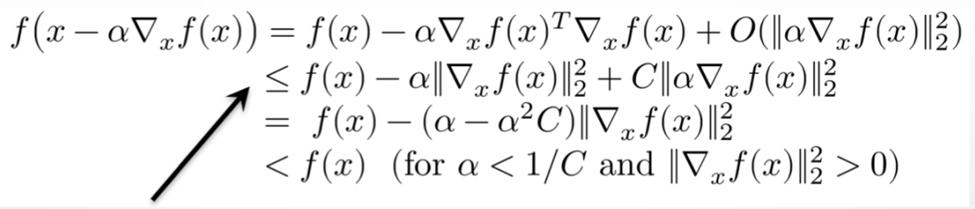
\includegraphics[width=\textwidth]{source/gradient-descent-proof.png}
    \label{fig:descent-gradient-proof}
\end{figure}

دقت کنید در خط اول صرفا نقطه جدید را در بسط تیلور تابع قرار دادیم.